\section{Implementation}
\label{sec:implementation}

In this section, we describe the implementation of the toolset.
\cite{listenmaa_claessen2015} presents the SAT encoding of the rules, when applied to an existing text.
Since we want to test the rules in a way that doesn't depend on data, we create a \emph{symbolic sentence}: a word sequence which we can modify according to the properties we want to test.
These words are combinations of tags
In order to create words with real ambiguities, we use a morphological lexicon
This sentence consists of symbolic words, which we c
In addition, we use a morphological lexicon to create symbolic words that contain real ambiguities.

\paragraph{SAT encoding of CG rules}

A single CG rule is a template which creates a concrete clause for each instance where it is applied.
%Each potential analysis is represented as a variable, and the rules are translated into clauses that operate on those variables.
Table~\ref{table:vars} shows the rule \texttt{REMOVE v IF (-1 det)} applied to the text \emph{the bear}.
The analyses of the word forms are represented as variables, and
the default rule ensures that each word has at least one analysis.
%This makes \texttt{the\_det} true by default, therefore the implication must hold, and \texttt{bear\_v\_pl} will be removed.
For more details about the encoding, see \cite{listenmaa_claessen2015}.

%As shown in table~\ref{table:vars}, \texttt{bear\_n\_sg} represents the possibility that \emph{bear} is a noun, and \texttt{bear\_v\_pl} 
%The rules are translated into clauses; one for each concrete application.
%Table~\ref{table:vars} shows the translation of the analyses to variables, and rules to clauses. See \cite{listenmaa_claessen2015} for further description.

% table:vars moved to main file for positioning


\paragraph{Word-internal constraints}

The symbolic sentence consists of symbolic words.
They are combinations of tags, and they may be underspecified---similarly, a given CG rule may target any noun, a plural noun or the noun \emph{bear}.
Given a large morphological lexicon, we can restrict each individual word to contain only realistic ambiguities. We map each word form in the lexicon to its possible analyses, and then ignore the actual word forms. For instance, a Spanish morphological lexicon contains the entries \texttt{casa:casar<verb><sg><p3>} and \texttt{casa:casa<noun><sg>}, hence we know that a confusion between a 3rd person singular verb and a singular noun is possible. 
%The lexicon is not likely to contain a wordform that can be analysed both as an adjective and punctuation, so that kind of ambiguous word is never created.

%However, since our method is corpus-free, we don't add any external restrictions as to what words can follow each other.

\paragraph{Symbolic sentences}

When we start applying rules, we need to have a sentence to which to apply.
As this is a corpus-free method, we don't have one.
Instead, we create a \emph{symbolic sentence}: sequence of words that can, in the beginning, have any tag combination.
At the word level, these tag combinations are restricted to only contain realistic ambiguities, as described in the previous paragraph.
At the sentence level, applying rules will start shaping the sentence.
An indeterminate blob of possible words undergoes rules that describe illegal sequences of analyses,
and at the application of each rule, more and more possibilities are discarded.

All rules are applied to all word, given that their context is in scope: for instance, the sentence-initial word doesn't meet any condition that requires something of previous words.
However, being a condition for another target will also shape a word.
At a level of real texts, a rule such as \texttt{REMOVE verb IF (-1 det)} is an instruction to remove a \texttt{verb} if we find a \texttt{det} before it.
In case of a symbolic sentence, we start in a situation where every word can be a \texttt{det} or a \texttt{verb}. In that context, the rule behaves as a broader constraint about every pair of two words \texttt{verb} may not follow \texttt{det}. This relation is encoded between all adjacent words, and each of them can follow the restriction in the way that is compliant with other rules.

\begin{figure}[]

\includegraphics[width=0.42\textwidth]{symbolic_sentence.png}

\caption{Symbolic sentence beginning to take shape}
\label{fig:example}
\end{figure}


% For instance, word 1 may be constrained by another rule to have no \texttt{det}, and this means that word 2 is free to have \texttt{verb} or not have it. If word 3 is required to have a  \texttt{det}, then word 4 either has to have no \texttt{verb}, or it has to have only \texttt{verb}, by the rule that the last analysis of the word will not be removed.

The applications of these rules shape our symbolic sentence into containing only things that can survive the rules. This means that we can ask a question ``after applying rules $0-i$, is it possible for $i+1$ to apply?'', and the answer is reliable; we can not find a counterexample by just having a bit more data, because we start from literally all possibilities, and each rule
restricts the set of possible sentences.

Note that this method is not suitable for language generation: rules in any realistic CG are tailored for real life ambiguities, whereas our symbolic sentence starts with literally all possibilities of tag combinations.

\paragraph{What kind of questions we can ask?}

The example so far has been of type ``Can rule Z apply after A-Y?''

We can construct all kinds of symbolic sentences. We can set the length, restrict individual words (e.g. ``3rd word must be a noun''), require that it triggers some rule but not other.
In case of a conflict, we can dig into the conflict and refine where the problem is: e.g. is the condition not met, or is it the case that the target is already removed or the only remaining analysis.




